\graphicspath{{images/}}

%%%%%%%%%%%%%%%%%%%%%%%%%%%%%%%%%%%%%%%%%%%%%%%%%%%%%%%%%%%%%%%%%%%%%%%%%%%%%%
% This is a chapter file (without title page and contents) on bivariate stable
% functions and directional Tukey depth. It emphasizes the key formulas – especially
% the optimal threshold \(s_{\max}\) – within the integral representation of the depth
% function. For further context see, e.g., \cite{rousseeuw1999depth}[1].
%%%%%%%%%%%%%%%%%%%%%%%%%%%%%%%%%%%%%%%%%%%%%%%%%%%%%%%%%%%%%%%%%%%%%%%%%%%%%%
\chapter{Bivariate Stable Functions and Directional Depth}

\section{Bivariate Stable Functions and Directional Depth}

In this chapter we study bivariate independent stable random variables and explore the directional depth function in a new light. Recall that we consider a symmetric stable random variable 
\[
X \sim S(\alpha,0,1,0)
\]
with characteristic function 
\[
\varphi_X(t)=\exp(-|t|^\alpha).
\]
Let \(X\) and \(Y\) be independent copies. Then, for any fixed constants \(a,b\), the linear combination
\[
Z = aX + bY
\]
has characteristic function
\[
\varphi_Z(t)=\exp\Bigl[-\Bigl(|a|^\alpha+|b|^\alpha\Bigr)|t|^\alpha\Bigr],
\]
implying that
\[
Z \sim S\Bigl(\alpha,0,\;c',\;0\Bigr),\quad\text{with}\quad c'=\Bigl(|a|^\alpha+|b|^\alpha\Bigr)^{1/\alpha}.
\]
This scaling property lets us standardize the problem so that
\[
P\Bigl(aX+bY\ge au+bv\Bigr)=P\Biggl(\frac{aX+bY}{c'}\ge\frac{au+bv}{c'}\Biggr).
\]
For brevity we set
\[
c=\frac{au+bv}{c'},
\]
which represents the standardized directional threshold.

\medskip
In our discussion the direction \((u,v)\) is always taken as a unit vector (with respect to the chosen norm). This is analogous to the treatment in \cite{rousseeuw1999depth}. 

\subsection{Analysis of the Directional Threshold Function and its Optimization}

We study the directional threshold function defined by
\[
c(a,b) = \frac{a\,u + b\,v}{\bigl(|a|^\alpha + |b|^\alpha\bigr)^{1/\alpha}},
\]
where the direction \((u,v)\) is assumed to be a unit vector and the weights \((a,b)\) are chosen under the normalization, since \(c(a, b)\) is homogeneus of degree 1.
\[
|a|^\alpha + |b|^\alpha = 1.
\]
A convenient parameterization is
\[
a = t^{1/\alpha},\quad b = (1-t)^{1/\alpha},\quad t\in[0,1],
\]
so that the function becomes
\[
c(t) = u\,t^{1/\alpha} + v\,(1-t)^{1/\alpha}.
\]

\medskip
\textbf{Concavity versus Convexity.}  
The nature of the mapping \(x \mapsto x^{1/\alpha}\) is crucial:
\begin{itemize}
  \item For \(\alpha>1\): Since \(1/\alpha < 1\), the function \(x^{1/\alpha}\) is \emph{concave}. Thus, \(c(t)\) is a concave function on \([0,1]\), and its maximum is attained at a unique interior point.
  \item For \(0 < \alpha \le 1\): Here, \(1/\alpha \ge 1\) so that \(x^{1/\alpha}\) is \emph{convex}; hence, \(c(t)\) is convex on \([0,1]\) and the maximum is attained at an endpoint.
\end{itemize}

\medskip
\textbf{Optimization for Different \(\alpha\) Cases.}

\subsubsection*{Case 1: \(\alpha > 1\)}

Differentiating \(c(t)\) and setting \(c'(t)=0\) leads quickly to
\[
\left(\frac{1-t}{t}\right)^{\frac{\alpha-1}{\alpha}} = \frac{v}{u},
\]
which yields the optimal value
\[
t^* = \frac{1}{1+\Bigl(\frac{v}{u}\Bigr)^{\frac{\alpha}{\alpha-1}}}.
\]
Substituting \(t^*\) into \(f(t)\) we obtain
\[
c_{\max} = u \left[1+\left(\frac{v}{u}\right)^{\frac{\alpha}{\alpha-1}}\right]^{\frac{\alpha-1}{\alpha}}.
\]
Defining
\[
\beta = \frac{\alpha}{\alpha-1},
\]
this simplifies to the elegant form
\[
\boxed{c_{\max} = \left(u^\beta + v^\beta\right)^{1/\beta}.}
\]

\subsubsection*{Case 2: \(0 < \alpha \le 1\)}

When \(0<\alpha\le1\) the function \(c(t)\) is convex, and therefore its maximum is attained at one of the endpoints of the interval. Hence, in this case we have
\[
\boxed{c_{\max} = \max\{u,v\}.}
\]


\section{Integral Representation for the Depth Function}

Once the threshold \(s_{\max}\) is determined, we evaluate the tail probability of a standard symmetric stable variable as follows. For 
\[
X\sim S(\alpha,0,1,0),
\]
the Gil–Pelaez inversion formula states that the CDF is
\[
F(x)=\frac{1}{2}+\frac{1}{\pi}\int_0^{\infty}\frac{\sin(tx)}{t}\exp(-t^\alpha)\,dt.
\]
Thus, the tail probability becomes
\[
P(X\ge x)=1-F(x)= \frac{1}{2}-\frac{1}{\pi}\int_0^{\infty}\frac{\sin(tx)}{t}\exp(-t^\alpha)\,dt.
\]

In our bivariate framework, after standardizing the linear combination with the scale factor \(c'=\bigl(|a|^\alpha+|b|^\alpha\bigr)^{1/\alpha}\) and using the directional threshold \(au+bv\), the probability of interest is
\[
P\Bigl(aX+bY\ge au+bv\Bigr)= P\Bigl(X\ge c\Bigr),
\]
where
\[
c=\frac{au+bv}{c'}.
\]

Plugging in the optimal threshold \(s_{\max}\) (which now depends on the relative values of \(u\) and \(v\) and on \(\alpha\)) we obtain the final formula for the depth:
\[
\boxed{
\operatorname{depth}(u,v)= P\Bigl(aX+bY\ge au+bv\Bigr)= \frac{1}{2}-\frac{1}{\pi}\int_0^{\infty}\frac{\sin\Bigl(t\,s_{\max}\Bigr)}{t}\exp(-t^\alpha)\,dt.
}
\]
Here, note that:
\begin{itemize}
  \item For \(\alpha>1\): \(s_{\max}=\left(u^\beta+v^\beta\right)^{1/\beta}\) with \(\beta=\frac{\alpha}{\alpha-1}\).
  \item For \(0<\alpha<1\): \(s_{\max}=\max\{u,v\}\).
\end{itemize}

\section{Special Cases and Depth Contours and Visualization}

For illustration, consider two scenarios:
\begin{itemize}
  \item When \(0<\alpha<1\) (say, \(\alpha=0.8\)), the function \(f(t)= u\,t^{1/\alpha}+v\,(1-t)^{1/\alpha}\) is convex so that the maximum is attained at one of the endpoints. Hence, the optimal threshold is
  \[
  s_{\max} = \max\{u,v\}.
  \]
  \item When \(\alpha>1\) (say, \(\alpha=1.3\)), the optimum is given by
  \[
  s_{\max} = \left(u^\beta+v^\beta\right)^{1/\beta},\quad \beta=\frac{1.3}{1.3-1}\approx 4.33.
  \]
\end{itemize}

Figure~\ref{fig:depth_08} shows the depth contours for \(\alpha=0.8\) and Figure~\ref{fig:depth_13} illustrates the contours for \(\alpha=1.3\). Notice that for \(\alpha>1\) the contours are given by the \(L^\beta\)-norm and tend to be rounder, while for \(\alpha<1\) the depth depends solely on the larger coordinate, leading to more “degenerate” contour shapes.

These examples also "prove" that our formulation is consistent with classical cases: for \(\alpha=1\) (the Cauchy case) one obtains \(s_{\max}=\max\{u,v\}\) and a tail probability of
\[
P(X \ge x)=\frac{1}{2}-\frac{1}{\pi}\arctan(x),
\]
and for \(\alpha=2\) (the Gaussian case) with \(\beta=2\), the threshold becomes
\[
s_{\max}=\sqrt{u^2+v^2},
\]
which is the familiar Euclidean norm. These special cases along with the contour plots vividly illustrate the rich geometric behavior of the depth function as \(\alpha\) varies.

\begin{figure}[htbp]\
    \centering
    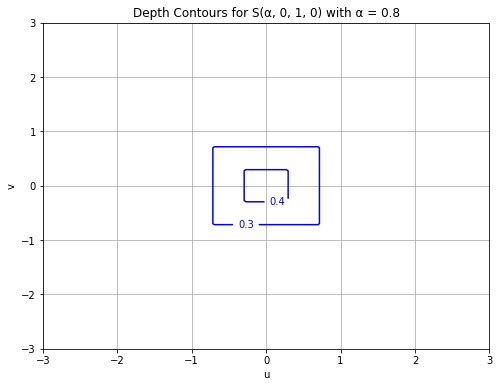
\includegraphics[width=\linewidth]{depth_08.png}
    \caption{Depth contours for $\alpha=0.8$.}
    \label{fig:depth_08}
  \end{figure}

  \begin{figure}[htbp]
    \centering
    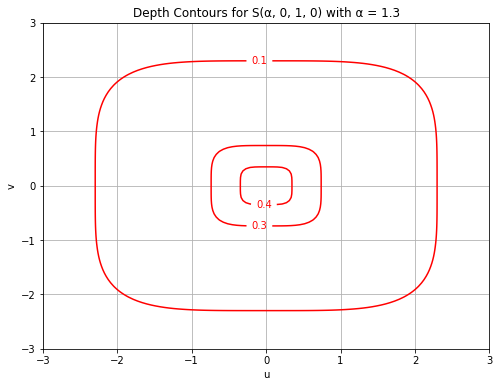
\includegraphics[width=\linewidth]{depth_13.png}
    \caption{Depth contours for $\alpha=1.3$.}
    \label{fig:depth_13}
  \end{figure}

%%%%%%%%%%%%%%%%%%%%%%%%%%%%%%%%%%%%%%%%%%%%%%%%%%%%%%%%%%%%%%%%%%%%%%%%%%%%%%
% Reference
%%%%%%%%%%%%%%%%%%%%%%%%%%%%%%%%%%%%%%%%%%%%%%%%%%%%%%%%%%%%%%%%%%%%%%%%%%%%%%
\begin{thebibliography}{1}
\bibitem{rousseeuw1999depth} Rousseeuw, P. J., \& Ruts, I. (1999). The depth function of a population distribution. \emph{Metrika}, 235--236.
\end{thebibliography}

\end{document}